\begin{marginfigure} % MARGIN FIGURE
%\captionsetup[subfigure]{labelformat=empty}
\subfloat[]{\margingraphics{figures/figsketch1a}}

\subfloat[]{\margingraphics{figures/figsketch1b}}

\subfloat[]{\margingraphics{figures/figsketch1}}
\caption{Sketching $f$ in Example~\ref{Ex:3.2.Eg6}.}
\label{fig:sketch1}
\end{marginfigure}

\begin{example} \label{Ex:3.2.Eg6}
Sketch $f(x) = 3x^3-10x^2+7x+5$.

\solution We follow the steps outlined in the Curve Sketching Concept.
\begin{enumerate}[1)]
\item The domain of $f$ is the entire real line; there are no values $x$ for which $f(x)$ is not defined.
\item Find the critical values of $f$. We compute $\fp(x) = 9x^2-20x+7$. Use the Quadratic Formula to find the roots of $\fp$:
$$x = \frac{20\pm \sqrt{(-20)^2-4(9)(7)}}{2(9)} = \frac19\left(10\pm\sqrt{37}\right) \Rightarrow x\approx 0.435, 1.787.$$

\item Find the possible points of inflection of $f$. Compute $\fpp(x) = 18x-20$. We have $$\fpp(x) = 0 \Rightarrow x= 10/9 \approx 1.111.$$

\item There are no vertical asymptotes.
\item We determine the end behavior using limits as $x$ approaches $\pm$infinity.				
$$\lim_{x\to -\infty} f(x) = -\infty \qquad \lim_{x\to \infty}f(x) = \infty.$$
We do not have any horizontal asymptotes.

\item We place the values $x=(10\pm\sqrt{37})/9$ and $x=10/9$ on a number line, as shown as shown below. We mark each subinterval as increasing or decreasing, concave up or down.

\begin{center}
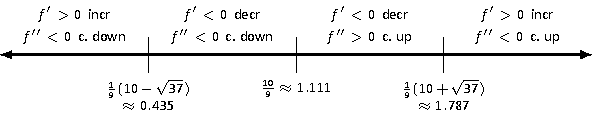
\includegraphics[scale=.75]{figures/figsketchline1}
\end{center}

\item We plot the appropriate points on axes as shown in Figure~\ref{fig:sketch1}-(a) and connect the points with straight lines. In Figure~\ref{fig:sketch1}-(b) we adjust these lines to demonstrate the proper concavity. Our curve crosses the $y$ axis at $y=5$ and crosses the $x$ axis near $x=-0.424$. In Figure~\ref{fig:sketch1}-(c) we show a graph of $f$ drawn with a computer program, verifying the accuracy of our sketch.
\end{enumerate}
\end{example}